\documentclass[conference]{IEEEtran}
\IEEEoverridecommandlockouts
% The preceding line is only needed to identify funding in the first footnote. If that is unneeded, please comment it out.
\usepackage{soul}
\usepackage{amssymb,amsmath,bm}
\usepackage{graphics,adjustbox}
\usepackage{tikz}
\usepackage{subfigure}
\usepackage{epstopdf}
\epstopdfsetup{suffix={}}
\usepackage{siunitx}
\sisetup{unitsep = \cdot}

\usepackage[figuresright]{rotating}
\usepackage[colorinlistoftodos]{todonotes}
\usepackage[english,algo2e,algoruled,vlined,linesnumbered]{algorithm2e}   % package for algorithm
\usepackage{enumerate}

\usepackage{easyReview}
\newtheorem{assumption}{Assumption}


\DeclareMathOperator*{\argmin}{arg min}

\def\BibTeX{{\rm B\kern-.05em{\sc i\kern-.025em b}\kern-.08em
    T\kern-.1667em\lower.7ex\hbox{E}\kern-.125emX}}
\begin{document}

\title{A Novel Model-Free Learning Approach for Dynamic Target Tracking Problem and its Validation using Virtual Robot Experimentation Platform 
%  
% \thanks{This work was supported in part by the Bradley University’s Caterpillar fellowship grant.}
}

\author{%~
\IEEEauthorblockN{Amr Elhussein and Md Suruz Miah}
\IEEEauthorblockA{\textit{Electrical \& Computer Eng.} \\
\textit{Bradley University}, Peoria, Illinois, USA \\
 aelhussein@mail.bradley.edu and smiah@bradley.edu}
% \and
% \IEEEauthorblockN{Fazel Keshtkar}
% \IEEEauthorblockA{\textit{Div. of Computer Science, Math. and Science} \\
% \textit{St John's University}, Queens, NY, USA \\
% keshtkaf@stjohns.edu}
% \and
% \IEEEauthorblockN{Mohammed Abouheaf}
% \IEEEauthorblockA{\textit{School of EECS} \\
% \textit{Univ. of Ottawa}, Canada\\
% mabouhea@uottawa.ca}
%
}

\maketitle

\begin{abstract}
  %

This paper advances the previous work done by authors by validating a model-free actor-critic reinforcement learning approach to solve dynamic target tracking problem for a car-like mobile robot. The learning approach generates the linear velocity and steering angle of the robot and it does not require any prior knowledge of the dynamic model of the moving target. Policy iteration approach is employed through Bellman's principle of optimality to assess the cost of the control actions derived by the proposed learning method. The algorithm is tested by coducting a set of computer experiments for complex secnarios using virtual robot expirementation platform widely known as CoppeliaSim.        

\todo[inline]{Review and expand}  
%
\end{abstract}

\begin{IEEEkeywords}
Leader-follower formation, mobile robots, reinforcement learning, policy iteration, trajectory tracking
\end{IEEEkeywords}

% \begin{nomenclature}
% \begin{deflist}[A]
% \defitem{ADP} \defterm{Approximate dynamic programming}
% \defitem{AL}\defterm{Approximate linearization}
% \defitem{RL}\defterm{Reinforcement learning}
% \end{deflist}
% \end{nomenclature}

\section{Introduction}
\label{sec:introduction}
\todo[inline]{Need to discuss in details the limitations of previous work, we
  can also add RL applications to robotics navigation}

Tracking a random moving target using a mobile robot, for instance, is a challenging task. This is mainly due to their inherent complex nonlinear dynamics dynamics. Most of the target tracking algorithms proposed in the literature either rely on A) complex mathematical models, B) simplified mathematical models, and C) nonlinear control techniques or driven by large amount of mostly offline data that leads to an overwhelming degree of computational complexity.


Over the past years mobile robots has been used in several applications in commercial and military sectors such as surveillance, search and rescue missions,coverage optimization, cooperative localization and dynamic target tracking tasks. In all of these mentioned applications a fleet of robot i.e agents interact with each other to achieve a certain goal. Leader-Follower or dynamic target tracking problem has recieved an extensive amount of study and research in the world of cooperative control theory due to it's wide promising applications such as search and rescure missions, wildlife monitoring and survillance to name a few . In a typical leader follower formation a number of robots referred to as followers apply local control actions to follow leader's robots in a specific predefined path such as \hl {cyclic, circular motion and time varying communication topologies.} \hl {limitations of other methods} many control methods were proposed however they have had the following limitations:
\\(1) a static leader/target is used.
\\(2) the leade/target's location or dynamic model is predetermined.  
\\(3) expensive hardware platforms are used to achieve the mobile target tracking. 
 \\The main contribution of this work is the development of a model-free learning approach to control the follower robot by which it overcome many of the limitations mentiond above as it does not rely on any prior information of the mathmetical model or the dynamic model. The steering angle and the linear speed of the follower robot are determined by collecting the position and orientation of both the leader and the follower. This set of information is gathered online over a finite period of time. The optimal control actions are then generated by utilizing Bellman's principal of optimality which acts as model free-reinfocment learning approach that allows the follower robot to follow the path of the leader while oviding collision by maintaining a safe distance. In this paper the proposed algorithm is further validated using a commercially available robot simulator, CoppeliaSim. This paper acts as first milestone in generalizing the algorithm to solve more sophisticated problem such as coverage and mapping. \hl{cite area coverage papers}
 \\The rest of the paper is orgnized as follows. Section II lays down the problem setting of the leader follower problem and mathemetical models of the robots and the state error. The model free actor-critic reinforcment learning and its key steps are described in section III.Section IV illustrates computer simulations for different secnarios that reflects the effectivness of the proposed method followed by conlusion and future work presented in section V.      

 

%\textit{\todo[inline]{Take some references from the following paragraphs}
%The task of localization and mapping in the context of leader-follower problems is very challenging. Such a task is becoming a ubiquitous  facet of modern life due to its promising application in addressing not only the leader-follower problem but also applicable in industry industry with heavy equipment trucks, in agriculture with autonomous crop maintenance, in home life with the autonomous vacuuming robot, along with research and design as seen in~\cite{Roberts2007,Durmus2015,Elara2014,HevrdejsKnoll2017-Indoor}.  In most leader-follower problem addressed in the literature to date, it is assumed that leader/target's position/state is known \textit{a priori}, which may not be the case in many applications such as tracking a mobile point source~\cite{Xu2013}. Furthermore, the localization and mapping task is of a paramount importance in addressing the problem of mobile target tracking, which has a number of promising applications, such as robotic navigation, search and rescue mission, wildlife monitoring, autonomous surveillance, to name a few. A large body of research has been conducted in the literature to address the localization and mapping problem. Relatively few papers have addressed the localization and mapping problem in the context of leader-follower tasks, where either (i) a static leader/target is used~\cite{Fernando2015}, (ii) the leader/target's location is predetermined, or (iii) expensive hardware platforms are used to implement the mobile target tracking strategy (see the work presented in~\cite{Yang2014}, for example). 
%
%The work done in this paper addresses some of the aforementioned issues by carrying out a cost-effective and easy-to-implement localization and mapping algorithm in the context of a leader--follower problem, a wheeled mobile robot is employed as a follower and a target moving on a two-dimensional (2D) plane is used as a leader. We emphasize that the position of the  leader is unknown to the follower robot \emph{a priori.} Therefore, the position and orientation of the follower robot and the position of the leader are to be simultaneously estimated while building the map of the environment of the robot using a set of networked wireless radio sensors placed on the ground. It is assumed that a radio sensor is mounted on the leader. The follower robot receives range measurements [herein the received signal strength indicator (RSSI) from radio sensors] from all radio sensors in its operating range. These measurements are then used to estimate the position and orientation of the follower robot, the 2D position of the leader, and the 2D positions of radio sensors placed in the robot's environment. Once the follower robot estimates its states (position and orientation) and the position of the leader, it moves towards the leader using the motion controller running onboard the follower robot. The design and implementation of the current work are based on the preliminary work of the robot navigation and mapping strategy conducted by the authors in~\cite{HevrdejsKnoll2017-Indoor,KnHeMi2017-c1,HeKnMi2017-c1}. Therefore, the main objective is to advance the work in~\cite{HevrdejsKnoll2017-Indoor,KnHeMi2017-c1,HeKnMi2017-c1} for a more general case, where a mobile robot is to follow a leader  whose position is unknown \emph{a priori.}   
%n}


\section{Dynamic target tracking and problem setting} 
\todo[inline]{Needs to reviewed}
 \label{sec:problemSetup}

Suppose that a wheeled mobile robot (follower) with coordinate $(x,y)$ and orientation $\theta\in[-\pi,\pi)~\si{\radian}$ with respect to the global X-Y coordinate has a linear speed $\nu$ and steering angle $\gamma$ which are considered as the two control actions. Let the posistion and orientation (pose) of the target i.e leader be ${\bf q}_k\equiv[x_k,y_k,\theta_k]$. The robot and the target are deployed in a 2D configuration in which the Follower is to follow the target trajectory defined by  $(\mathbf{p}_k^{[d]})^T=[x_k^{[d]},y_k^{[d]}(t)]$ at time $t\ge 0$ with $t=k \, T_s,$ $k\in\mathbb{N}_0,$ and $T_s>0$ being the sampling time. Note that this trajectory is completley random. The target motion is modeled by the following discrete-time system:
 \begin{align}
   \label{eq:leaderDT}
   \mathbf{p}_{k+1}^{[d]} = \mathbf{p}_k^{[d]} + T_s \, \mathbf{u}_k^{[d]},
 \end{align}  
with $\mathbf{u}_k^{[\ell]}\in\mathbb{R}^2$ being the control inputs of the target movment. 
\\ The follower robot is to maintain a constant safe-distance $d>0$ from target. The dynamic car-like model of the follower robot is defined as follows:
  \begin{figure}
   \centering
   \fcolorbox{gray!10}{gray!5}{
     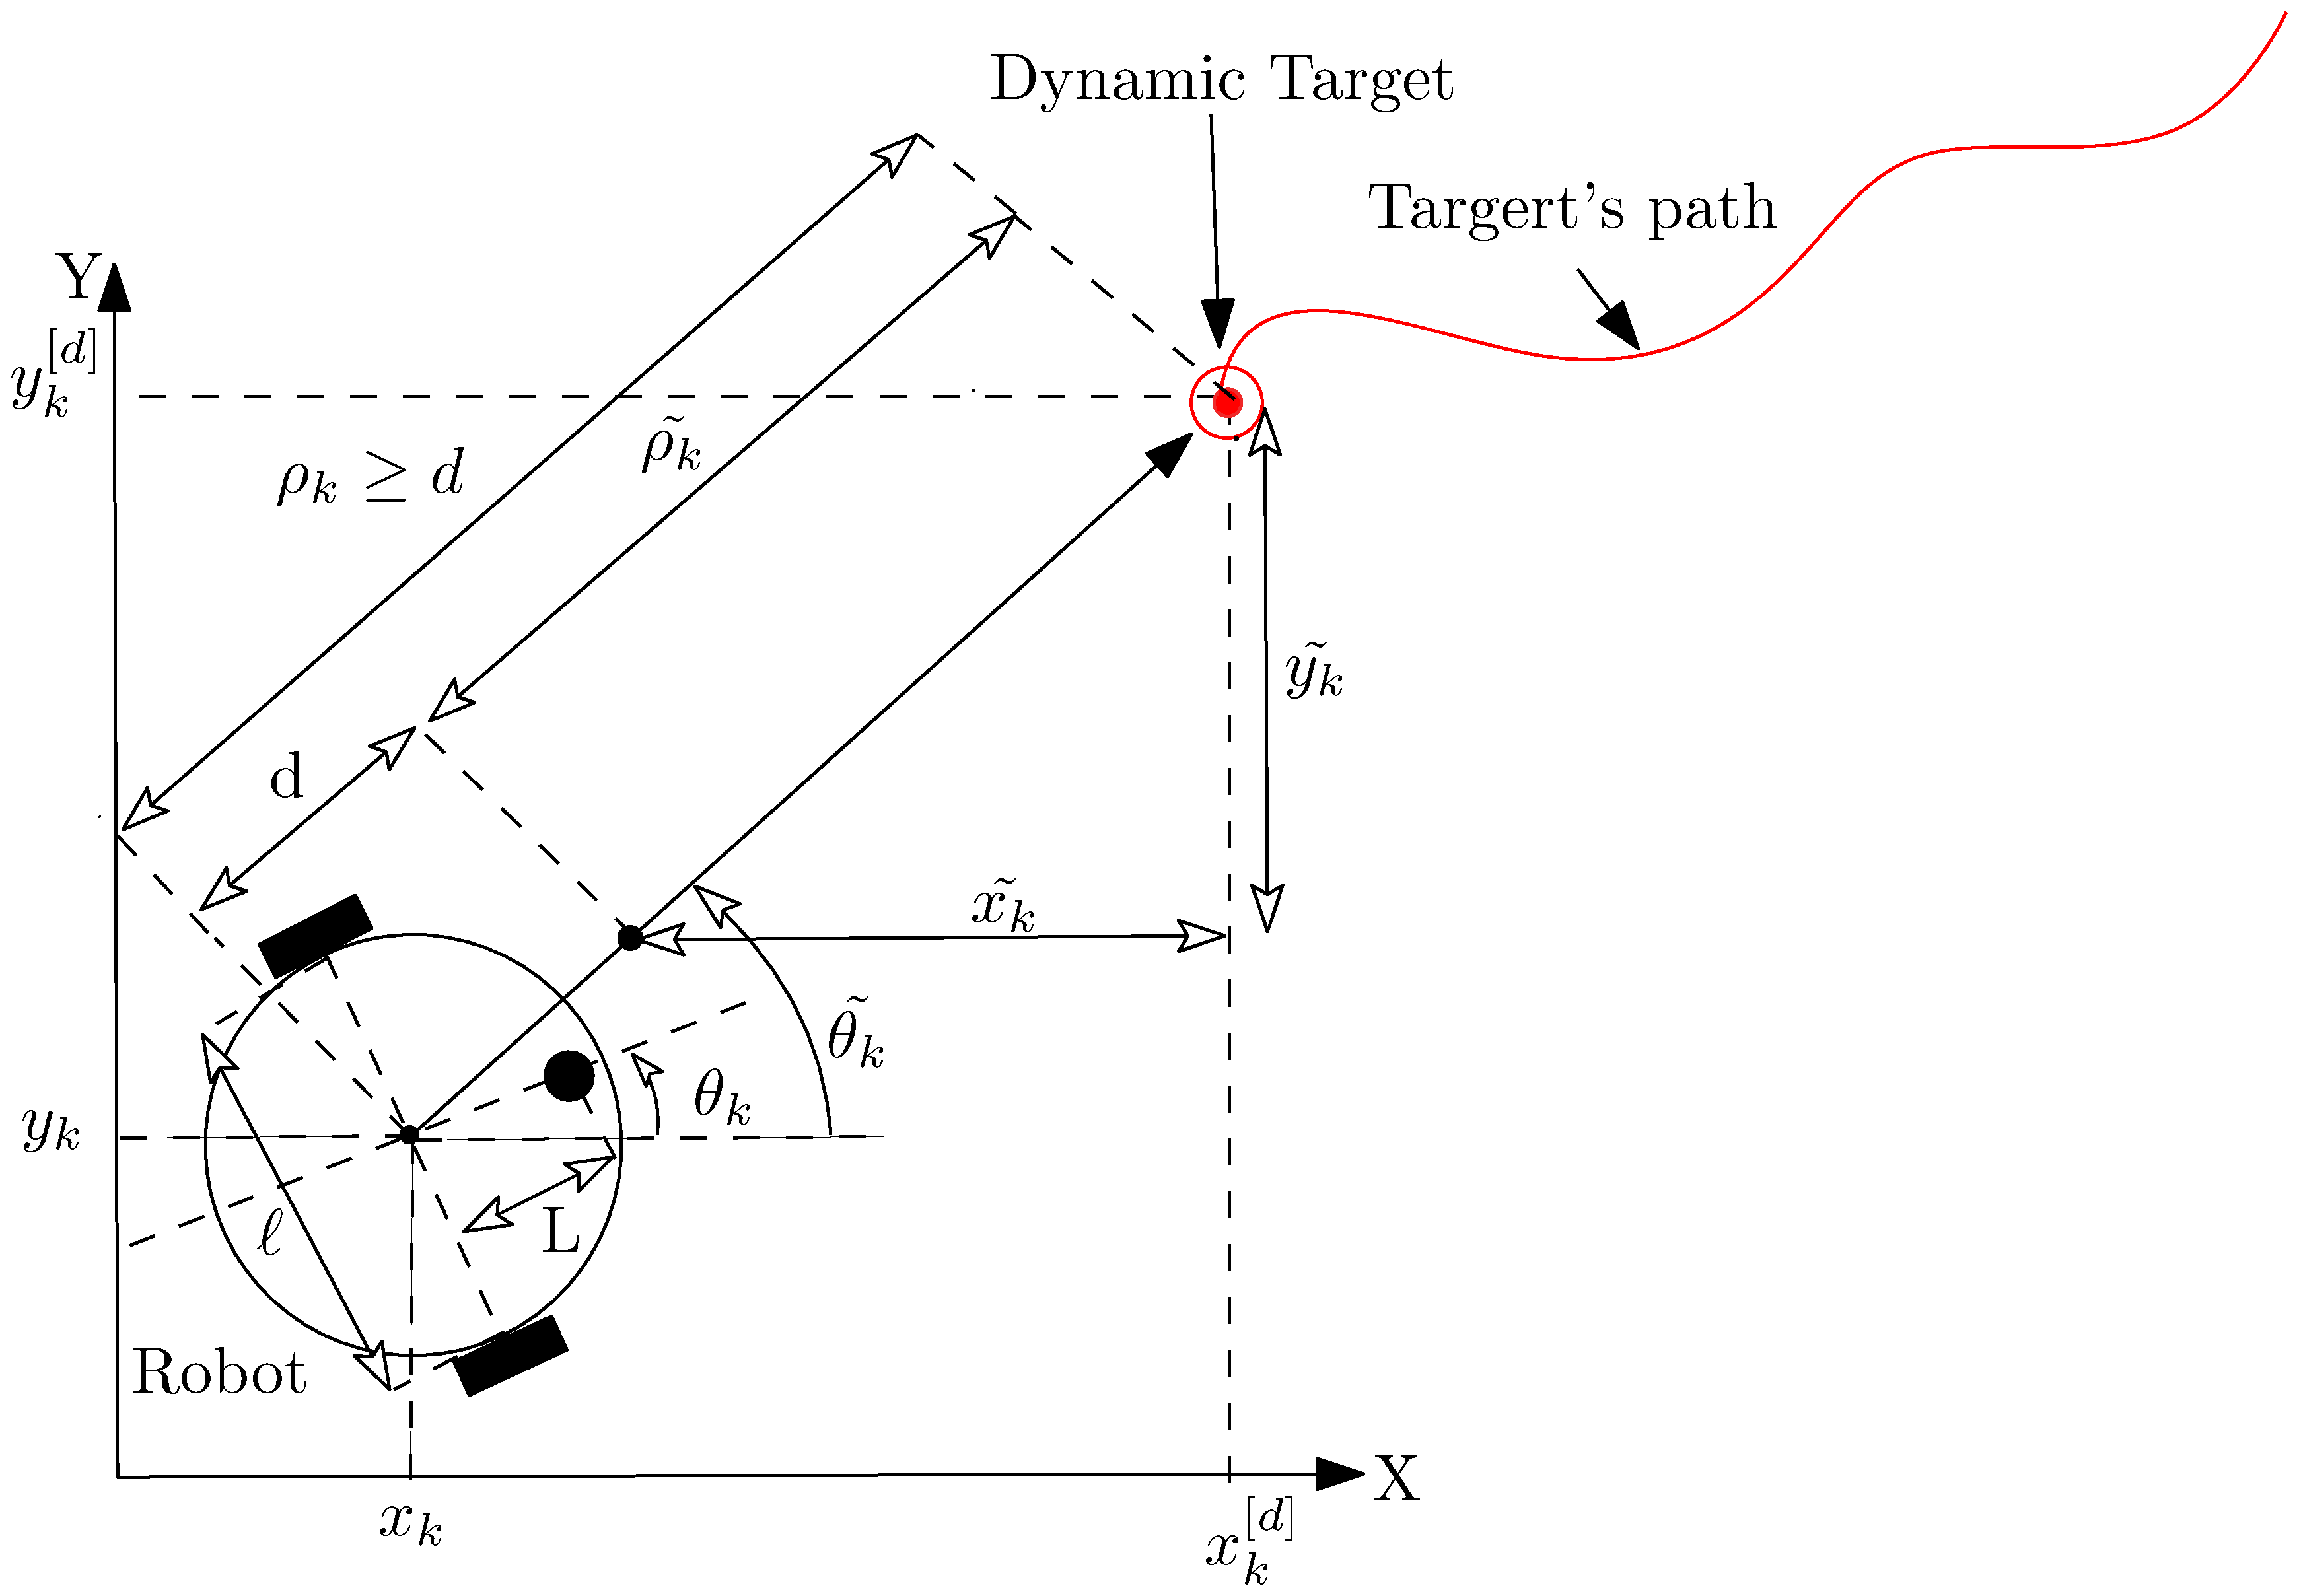
\includegraphics[width=0.45\textwidth]{figs/ipe/LFMICSetup.eps}
    }
   \caption{Mobile robot and its dynamic target tracking problem setup.}
   \label{fig:leaderFollowerSetup}
 \end{figure}
 \begin{subequations}
   \begin{align}
     x_{k+1}& =x_{k}+T_s\nu_{k}\cos{(\theta_{k}+\gamma_{k})} + \zeta_1,\\  
     y_{k+1}& =y_{k}+T_s\nu_{k}\sin{(\theta_{k}+\gamma_{k})}+ \zeta_2,\\
     \theta_{k+1}&=\theta_{k}+T_s\nu_{k}\frac{\sin{(\gamma_{k})}}{l}+ \zeta_3,
   \end{align}
 \label{eq:robotModel1-DT}
 \end{subequations}
 \\
\hl{Note that the follower dynamic model obeys Ackermann steering principle where $\gamma_k\in(-\frac{\pi}{2},\frac{\pi}{2})$ is the front wheel steering angle with respect to the robot's orientation $\theta_k\in[-\pi,\pi),$ $\nu_k$ is the linear speed, $l$ is the distance between the drive wheels of the robot, and $\zeta_1,\zeta_2,\zeta_3\in\mathbb{R}$ are the model uncertainties.} 
\\
We then define the error vector as:
 \begin{multline}
     \label{eq:stateError}
   \mathbf {e}_k^T = [\rho_e,\theta_e]^T =
   [\sqrt{x_e^2+y_e^2},\theta_e]^T = \\
   \begin{bmatrix}
     \sqrt{(x_k^{[d]} - x_k - d\cos\theta_k^{'})^2+
     (y_k^{[d]} - y_k - d\sin\theta_k^{'})^2},
     \theta_k^{'} - \theta_k
   \end{bmatrix},
 \end{multline}
 
 where $\theta_k^{'} = \mathrm{atan2}\left(y_k^{[d]}-y_k, x_k^{[d]}-x_k\right).$ and ${\rho_e}$ being the euclidean distance. 
\\
\hl{The control problem can then be formally stated as follows}: Find $\nu_k$ and $\gamma_k$ such that ${\bf e}_k\to {\bf 0}$ as  $k\to\infty$ subject to~\eqref{eq:leaderDT}~\text{and}~\eqref{eq:robotModel1-DT}.

%
%
%  In the next section, a conventional trajectory tracking method is investigated to solve the problem~\eqref{eq:problem}. This is followed by the proposed approximate dynamic programming technique which is illustrated in section~\ref{sec:solutionADP}.




\section{Proposed actor-critic RL Approach}
\todo[inline]{Needs to be rewritten}

 \label{sec:RLSolution}

 The solution of the leader-follower formation problem is realized using a reinforcement learning approach. It employs model-free strategies for solving a temporal difference equation developed herein. This solution is equivalent to solving the underlying Bellman optimality equation for  the dynamical error model~\eqref{eq:stateError}. The relative importance of the states in the error vector ${\bf e}_k$ and the control decisions (linear velocity and steering angle) of the follower-robot are evaluated using the  performance (cost) index: %
 \begin{align}
 \label{eq:costFunctional}
 J = \sum_{k=0}^\infty \frac{1}{2}\left[{\bf e}_k^T \, {\bf Q} \, {\bf e}_k + {\bf u}_k^T \, {\bf R} \, {\bf u_k}\right],
 \end{align}    
 where ${\bf Q}\in\mathbb{R}^{3\times 3}$ and ${\bf R}\in\mathbb{R}^{2\times 2}$ are symmetric positive definite weighting matrices. The objective of the optimization problem, following~\cite{Lewis2013-Reinforcement}, is to find an optimal sequence of control polices $\{\mathbf{u}^*_k\}_{k=0}^\infty$ that minimizes the cost index $J$ along the state-trajectories~\eqref{eq:leaderDT}~and~\eqref{eq:robotModel1-DT}. Motivated by the structure of the convex quadratic cost functional~\eqref{eq:costFunctional}, let the solution of the tracking control problem employ the value function $V({\bf e}_k,{\bf u}_k)$ defined by %
 %
 \begin{equation*}
 \label{eq:valueFunction}
 V({\bf e}_k,{\bf u}_k) = \sum_{\kappa=k}^\infty \frac{1}{2}\left({\bf e}_\kappa^T\, {\bf Q}\, {\bf e}_\kappa + {\bf u}_\kappa^T \, {\bf R}\, {\bf u_\kappa}\right).
 \end{equation*}
 %
 This structure yields a temporal difference form (i.e., Bellman equation) as follows
 \begin{equation*}
 \label{eq:tempraldiffeq}
 V({\bf e}_k,{\bf u}_k)= \frac{1}{2}\left[{\bf e}_k^T\, {\bf Q}\, {\bf e}_k + {\bf u}_k^T\, {\bf R}\, {\bf u_k}\right] +V({\bf e}_{k+1},{\bf u}_{k+1}).
 \end{equation*}
 %
 Applying Bellman's optimality principle yields the optimal control policies ${\bf u}_k^*,~k\ge 0,$ such that~\cite{Lewis2012} %
 %
 \begin{align*}
 {\bf u}^*_k = \argmin_{{\bf u}_k}\left[\frac{1}{2}\left[{\bf e}^T_k\,  {\bf Q}\, {\bf e}_k +{\bf u}^T_k\,  {\bf R} \,  {\bf u}_k\right]   +
 V({\bf e}_{k+1},{\bf u}_{k+1})\right].
 \label{eq:argMinControlAction}
 \end{align*}
 %
 Alternatively, this optimal  policy form is equivalent to ${\bf u}^*_k = \argmin_{{\bf u}_k}\left[
 V({\bf e}_{k},{\bf u}_{k})\right].$
 Therefore, the underlying Bellman optimality equation follows %
 %
 \begin{equation*}
 \label{eq:BellOpt}
 V^*({\bf e}_k,{\bf u}^*_k)= \frac{1}{2}\left[{\bf e}_k^T\, {\bf Q}\, {\bf e}_k + {\bf u}_k^{*T}\, {\bf R}\, {\bf u}^*_k\right] +V^*({\bf e}_{k+1},{\bf u}^*_{k+1}),
 \end{equation*}
 %
 where $V^*(\cdot,\cdot)$ is the optimal solution for Bellman optimality equation. This temporal difference equation is utilized by reinforcement learning process which solves the following temporal difference approximation form %
 %
 \begin{align}
 \hat{V}(\mathbf{z}_k) = \frac{1}{2}\mathbf{z}_k^T\, \bar{\mathbf{P}}\, \mathbf{z}_k + \hat{V}(\mathbf{z}_{k+1}),
 \label{eq:valueFunctionEstimated}
 \end{align}
 %
 where $\mathbf{z}_k = \left[\mathbf{e}_k ,\mathbf{u}_k\right]^T\in\mathbb{R}^5,$ $V\left(\mathbf{e}_k,\mathbf{u}_k\right) \approx \hat{V}(\mathbf{z}_k),$  and $\bar{\mathbf{P}}$ is a symmetric block-diagonal matrix formed using $(\mathbf{Q},\mathbf{R}),$~\textit{i.e.,~}$\bar{\mathbf{P}} = \mathrm{blockdiag}(\mathbf{Q},\mathbf{R}).$ %
 The approximation of the solving value function $\hat{V}(\mathbf{z}_k)$ employs a quadratic form so that $\hat{V}(\mathbf{z}_k)=\frac{1}{2}\mathbf{z}_k^T\, \mathbf{P}\, \mathbf{z}_k,$ where $\mathbf{P}\in\mathbb{R}^{5\times 5}$ is a positive definite matrix. Hence, the optimal control strategy $\mathbf{u}_k^*$ can be expressed as follows %
 %
 \begin{align}
 \label{eq:modelFreePolicy}    
 \mathbf{u}_k^* = \argmin_{\mathbf{u}_k}\left[\hat{V}(\mathbf{z}_k)\right] = -\,  \mathbf{P}_{uu}^{-1}\, \mathbf{P}_{ue}\, \mathbf{e}_k,
 \end{align}
 %
 where $\mathbf{P}_{uu}$ and $\mathbf{P}_{ue}$ are sub-blocks of symmetric matrix $\mathbf{P}.$ %   
 %

% A two-step solution mechanism that is based on policy iteration is employed to solve the temporal difference equation~\eqref{eq:valueFunctionEstimated} using the policy~\eqref{eq:modelFreePolicy}. First, the adaptive critics are used to approximate the solving value function $\hat V(\cdot)$ using a multi-layer critic neural network as shown in Fig.~\ref{fig:nnCritic}. %
 %
% \begin{figure}
%     \centering
%     \fcolorbox{blue}{gray!5}{
%         \begin{adjustbox}{max width = 0.45\textwidth}
%             \tikzset{%
%                 input neuron/.style={
%                     circle,
%                     fill=green!50,
%                     minimum size=0.7cm
%                 },
%                 neuron missing/.style={
%                     draw=none, 
%                     scale=1,
%                     fill=white,
%                     text height=0.01cm,
%                     execute at begin node=\color{black}$\vdots$
%                 },
%             }
%            
%%             \tikzset{%
%                 hidden neuron/.style={
%                     circle,
%                     fill=blue!50,
%                     minimum size=0.7cm
%                 },
%                 neuron missing/.style={
%                     draw=none, 
%                     scale=1,
%                     fill=white,
%                     text height=0.01cm,
%                     execute at begin node=\color{black}$\vdots$
%                 },
%
%             }
%            
%%             \tikzset{%
%                 output neuron/.style={
%                     circle,
%                     fill=red!50,
%                     minimum size=0.7cm
%                 },
%                 neuron missing/.style={
%                     draw=none, 
%                     scale=1,
%                     fill=white,
%                     text height=0.01cm,
%                     execute at begin node=\color{black}$\vdots$
%                 },
%             }
%            
%%             \begin{tikzpicture}[x=1.5cm, y=1.5cm]
%            
%%             \foreach \m/\l [count=\y] in {1,2,missing,3}
%             \node [input neuron/.try, neuron \m/.try] (input-\m) at (0,2.5-\y) {};
%            
%%             \foreach \m [count=\y] in {1,2,3,missing,4}
%             \node [hidden neuron/.try, neuron \m/.try ] (hidden-\m) at (2,2.5-\y*1.1) {};
%            
%%             \foreach \m [count=\y] in {1}
%             \node [output neuron/.try, neuron \m/.try] (output-\m) at (4,2.5-\y*2.8) {};
%            
%%             \foreach \l [count=\i] in {1,2,n+m}
%             \draw [<-] (input-\i) -- ++(-1,0)
%             node [above, midway] {$\mathbf{z}_{k,\l}$};
%            
%%             \foreach \l [count=\i] in {1,2,3,~\mbox{$\bar{n}$}}
%             \node [above] at (hidden-\i.north) {$\rho_{\l}$};
%            
%%             \foreach \l [count=\i] in {1}
%             \draw [->] (output-\i) -- ++(1,0)
%             node [above, midway] {$\hat{V}(\mathbf{z}_{k})$};
%             % node [above, midway] {$\hat{V}_\l$};
%            
%%             \foreach \i in {1,...,3}
%             \foreach \j in {1,...,4}
%             \draw [->] (input-\i) -- (hidden-\j);
%            
%%             \foreach \i in {1,...,4}
%             \foreach \j in {1}
%             \draw [->] (hidden-\i) -- (output-\j);
%            
%            
%            
%%             \foreach \l [count=\x from 0] in {Input, Hidden, Output}
%             \node [align=center, above] at (\x*2,1.9) {\l \\ layer};
%            
%%             \node [align=center, below] at (3,-2.5) {Weights \\ $\boldsymbol{\omega}$};
%             \draw[->,ultra thick](3,-2.5) -- (3,1.4);
%            
%%             \end{tikzpicture}
%         \end{adjustbox}      
%     }
%     \caption{Critic neural network structure for approximating value function.}
%     \label{fig:nnCritic}
%       \end{figure}
 %      
 Second, the policy evaluation step of this process updates the critic weights $\bm{\omega}$ in real-time without acquiring any formation about the dynamics of the leader or follower dynamical systems  (the calculation mechanism of the critic weighs $\boldsymbol{\omega}$ is explained later on). This is done to search for a strictly better policy. %
 %

% Note that, the policy iteration computational setup rearranges the temporal difference expression~\eqref{eq:valueFunctionEstimated} such that %
 %
 \begin{equation}
 \label{eq:const}
 \mathbf{z}_k^T\, \mathbf{P}\, \mathbf{z}_k - \mathbf{z}_{k+1}^T\, \mathbf{P}\, \mathbf{z}_{k+1} = \mathbf{z}_k^T\, \bar{\mathbf{P}}\, \mathbf{z}_k. 
 \end{equation}
 %
 This equation is utilized repeatedly in order to evaluate a certain policy during at least $\eta\ge \bar n, \bar n= (3+2)(3+2+1)/2$ evaluation steps (i.e., the lowest evaluation interval spans $k$ to $k+\bar n$ calculation samples) in order to update the critic weights vector  $\boldsymbol{\omega}=\mathrm{vec}(\mathbf{P}),$ which consists of connection weights between the neurons of the hidden layer and the output layer of the critic neural network shown in Fig.~\eqref{fig:nnCritic}. The operator $\mathrm{vec}(\mathbf{P})$ forms the columns of the $\mathbf{P}$ matrix into a column vector $\mathbf{\omega}$ of dimension $\bar{n}=15$ since the matrix $\mathbf{P}$ is a symmetric matrix. The left hand side of~\eqref{eq:const} is expressed using the following critic approximation form %
 %
 $$\hat{V}(\mathbf{z}_k)-\hat{V}(\mathbf{z}_{k+1})=\boldsymbol{\omega}^T\tilde{\bm{\rho}}(\mathbf{z}_{k,k+1}),$$
 %
 where $\tilde{\bm{\rho}}(\mathbf{z}_{k,k+1})=\bm{\rho}(\mathbf{z}_k)-\bm{\rho}(\mathbf{z}_{k+1}) \in \mathbb{R}^{15 \times 1}, \, \bm{\rho}(\mathbf{z}_k)=\left(\mathbf{z}^q_k\otimes\mathbf{z}^h_k\right)$ $(q=1,\dots, 5, \,\, h=q,\dots,5),$ and $\boldsymbol{\omega}^T = [0.5 \, P^{11},P^{12},P^{13},P^{14}, P^{15}, \, 0.5 \, P^{22}, P^{23},P^{24},P^{25},$ $\,0.5 \, P^{33}, P^{34},P^{35},\,0.5 \, P^{44},P^{45}, \,0.5 \, P^{55}]^T \in \mathbb{R}^{1\times 15}$ ($P^{ij}$ is the $ij^{th}$ entry of matrix $\mathbf{P}$). %
 %
 The critic weights $\boldsymbol{\omega}$ are updated using a gradient descent approach, where the tuning error $\varepsilon_k$ at each computational instance $k$ follows $\varepsilon_k =\boldsymbol{\omega}^T\tilde{\bm{\rho}}(\mathbf{z}_{k,k+1})-{v}_k,$ where $v_\kappa = \frac{1}{2}\mathbf{z}_{k}^T \, \bar{\mathbf{P}} \, \mathbf{z}_{k}$. As detailed earlier, it is required to perform at least $\eta \ge \bar n$ evaluation steps before updating the critic weights $\boldsymbol{\omega}$ (i.e., finding the new improved policy). Hence, it is required to minimize the sum of square errors such that %
 %
 \begin{multline*}
   \delta_c =\sum_{\kappa=0}^{\eta-1}\frac{1}{2}(\boldsymbol{\omega}^T\tilde{\bm{\rho}}(\mathbf{z}_{k+\kappa,k+\kappa+1})-{v}_{k+\kappa})^2 = \frac{1}{2}\| \mathbf{v} - \bm{\Lambda}\bm{\omega}\|^2\\
   =\frac{1}{2}\left(\mathbf{v} - \bm{\Lambda}\bm{\omega}\right)^T \left(\mathbf{v} - \bm{\Lambda}\bm{\omega}\right), 
 \end{multline*}
 where $\bm{\Lambda} = [{\bf o}_0,{\bf o}_1,\ldots,{\bf o}_{\eta-1}]^T \in \mathbb{R}^{\eta\times 15}$ with ${\bf o}_\kappa = \tilde{\bm{\rho}}^T({\bf z}_{k+\kappa, k+\kappa+1}) \in \mathbb{R}^{1\times 15}$ and ${\bf v} =[v_0,v_1,\ldots,v_{\eta-1}]^T \in \mathbb{R}^{\eta}$ with $v_\kappa = \frac{1}{2}\mathbf{z}_{k+\kappa}^T \, \bar{\mathbf{P}} \, \mathbf{z}_{k+\kappa}$ for $\kappa = 0,1,\ldots, \eta-1$. %
 Therefore, the update law of the critic weights using the gradient decent approach for at least $\bar n$ samples is given by %
 \begin{multline}
   \bm{\omega}^{[r+1]} = \bm{\omega}^{[r]} - \ell_c\frac{\partial\delta_c}{\partial \bm{\omega}} = \bm{\omega}^{[r]} - \ell_c\left(-\bm{\Lambda}^T\mathbf{v} + \bm{\Lambda}^T \bm{\Lambda}\bm{\omega}^{[r]}\right)\\ 
 =\bm{\omega}^{[r]} - \ell_c \bm{\Lambda}^T\left(\bm{\Lambda}\bm{\omega}^{[r]}-\mathbf{v}\right), 
 \label{eq:criticWeights}
 \end{multline}
 %
 where $0<\ell_c<1$ is a critic learning rate and $r$ is the  update index of the critic weights. 

% The newly computed critic weights $\boldsymbol{\omega}$ are used to reconstruct the matrix ${\bf P}$ (i.e., updating the solving value function and hence calculating the associated policy) such that 
 %
 \begin{center}
 ${\bf P}=\begin{bmatrix} 
 2\,\omega^{1}    & \omega^{2}      & \omega^{3}       & \omega^{4}       & \omega^{5} \\ 
 \omega^{2}       &2\, \omega^{6}   & \omega^{7}       & \omega^{8}       & \omega^{9} \\
 \omega^{3}       & \omega^{7}      &2\, \omega^{10}   & \omega^{11}      & \omega^{12} \\
 \omega^{4}       & \omega^{8}      & \omega^{11}      & 2\,\omega^{13}   & \omega^{14} \\
 \omega^{5}       & \omega^{9}      & \omega^{12}      & \omega^{14}      & 2\,\omega^{15}   
 \end{bmatrix}\in \mathbb{R}^{5\times 5},$
 \end{center}
 %
 where $\omega^{i}$ is the $i^{th}$ entry of the weight vector $\bm{\omega}.$ The complete policy iteration solution process for the leader-follower problem is detailed out in Algorithm \ref{alg:ModelFreeTracking}. %
 %
 \begin{algorithm2e}
     \caption{\label{alg:ModelFreeTracking} Model-free reinforcement learning using the policy iteration solution.}
     \DontPrintSemicolon
     \KwIn{Sampling-time $T_s,$ $\mathbf{Q},~\text{and}~\mathbf{R}$ }
     \KwOut{Error trajectory $\mathbf{e}_k,$ for $k=0,1,\ldots$}
     % \KwData{Map representation using occupancy grid technique}
     % \KwResult{output******************************}
     \Begin{
         $k=0, r = 0$ \tcc*[h]{Discrete time and policy indices}\;
         $\eta = (n+m)(n+m+1)/2$\;
         Initialize $\mathbf{P}^{[0]}$ \tcc*[h]{Positive definite}\;
                 Set offset distance $d$\;
                 Given approximate initial poses of leader and follower, compute $\mathbf{e}_0$ using error model~\eqref{eq:stateError}\;
                 Compute follower's input $\mathbf{u}_0^{[0]}$ using policy~\eqref{eq:modelFreePolicy}\;
         \Repeat(\tcc*[h]{Main timing loop}){Tracking errors are zero}
         {
             Find $\mathbf{e}_{k+1}$ using~\eqref{eq:stateError}\;
             Compute policy $\mathbf{u}_{k+1}^{[r]}$ using~\eqref{eq:modelFreePolicy}\;
             %Evaluate and record Equation~\eqref{eq:modelFreeMatrixSolution}\;
             \If{[$(k+1)~\mathrm{modulo}~\eta]==0$ }
             {
                 $r\leftarrow r+1$\tcc*[h]{Evaluate policy}\;
                 Solve for the critic-weights $\bm{\omega}$ using~\eqref{eq:criticWeights}\;
                 Construct matrix $\mathbf{P}^{[r]}$ using vector $\bm{\omega}$\;
 %                \eIf{$\|\mathbf{P}^{[r]} - \mathbf{P}^{[r+1]}\|<\varepsilon$}{Set $\mathbf{u}_{k+1}^*\leftarrow\mathbf{u}_{k+1}^{[r]}$}{$k\leftarrow k+1$ }
             }
 %        {
 %                $k\leftarrow k+1$
 %            }
         $k\leftarrow k+1$
         }
     }
 \end{algorithm2e}    
    
    


  

 \section{Computer Experiments and Results}
 \label{sec:resultsExperiments}
 This section adopts the theoritical results discussed in the previous section by simulating the Algorithm using the Pioneer 3-DX in CoppeliaSim. The results obtained by the authors in \hl{cite flairs paper here} are validated using the commercial robot simulator, CoppeliaSim as a prelminary step to implement the Algorithm experimantally in real world. we present the dynamics of the tracking error and the convergence characterisitcs of the actor and critic weights. The weighting matrices are set to $\mathbf{Q} = \mathrm{diag}[0.001,0.001]$ and $\mathbf{R} = \mathrm{diag}[10^{-5}, 10^{-5}].$ % 
  \[Q=0.001 
  \begin{bmatrix}
  1       & 0   \\
  0       & 1   \\
  \end{bmatrix},
  R=0.00001
  \begin{bmatrix}
  1       & 0 \\
  0       & 1 
  \end{bmatrix}.\]
 The actor and critic learning rates $\ell_c$ are set to  $0.01$ and $0.0001$. The sampling time $T_s$ is set to $0.001 \sec.$ The desired distance offset between the leader and the follower is set to $ d = 0.5$ [m] for all scenarios.
 The CoppeliaSim simulator accuratly mimic what would happen in a realworld scenario following idustry standatrds and guidlines. The Pioneer robot model and the  was initally placed at position (-1,-2.5) m.The Target modeled as a cylinder was initially positioned on a random position around the origin (0,0). The simulation was run for 
\begin{figure}
   \centering
   \fcolorbox{gray!10}{gray!5}{
     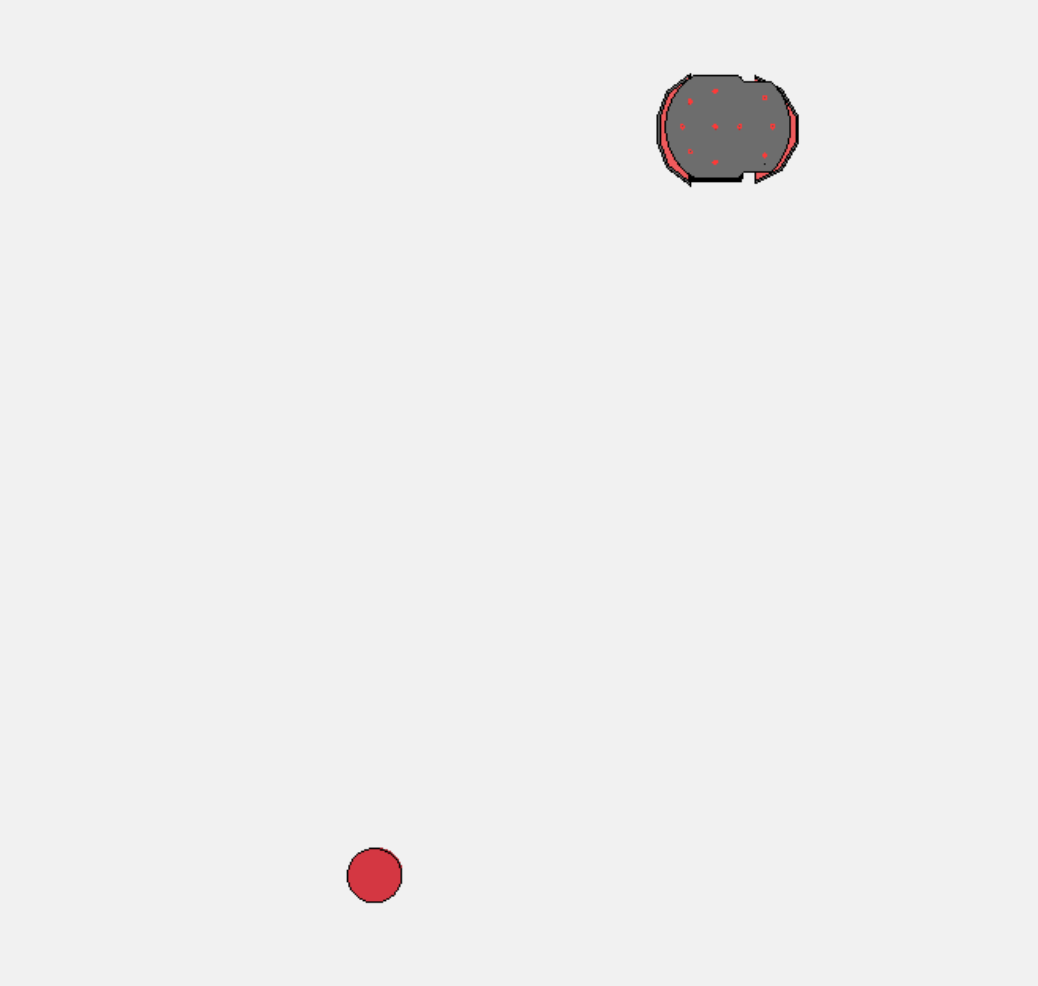
\includegraphics[width=0.45\textwidth]{figs/coppeliasim.png}
`     }
   \caption{CoppeliaSim Scene.}
   \label{fig:CoppeliaSim Scene}
 \end{figure}  
    
 \begin{figure*}[htbp]%
 \subfigure[][]{%
    \label{fig:trajectoryRandom}%
    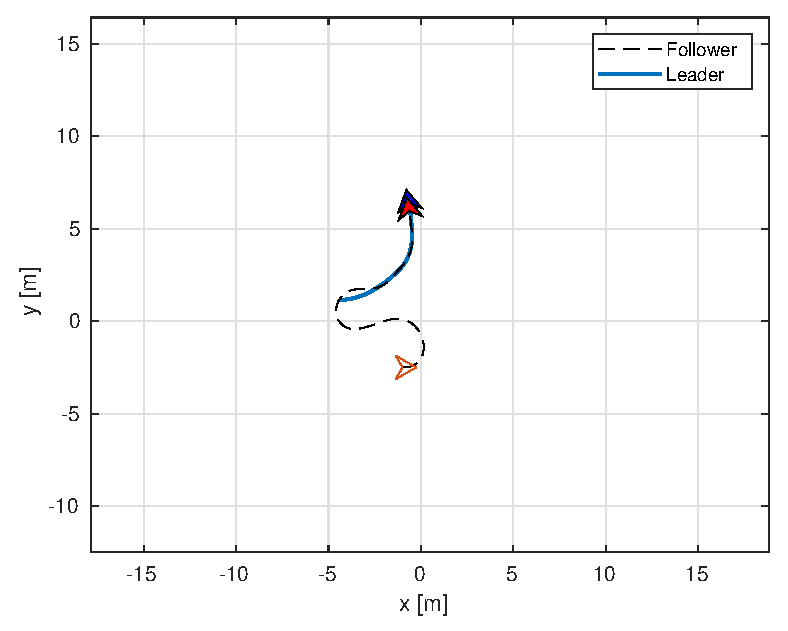
\includegraphics[width=0.48\textwidth,height=0.25\textheight]{figs/coppelia/firstScenario/trajectoryRandomPathDistance.eps} }
\subfigure[][]{%
    \label{fig:stateErrorRandom}%
    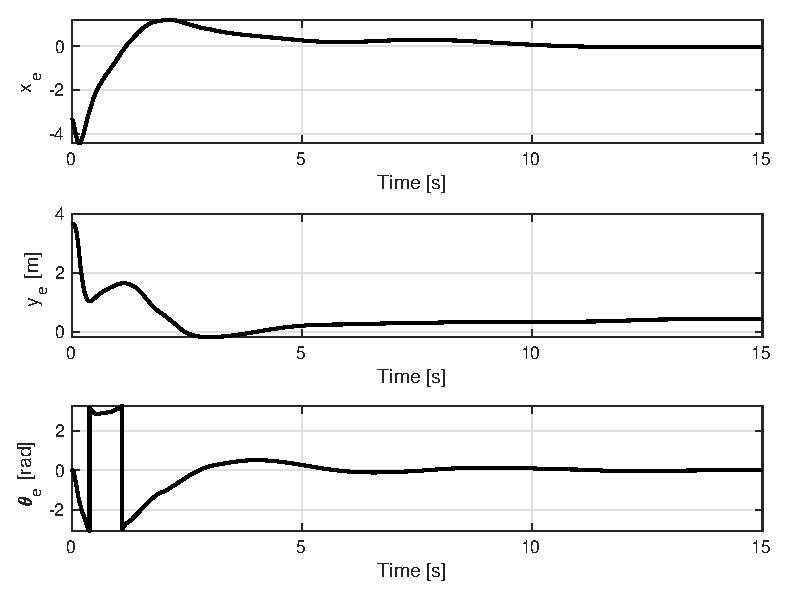
\includegraphics[width=0.48\textwidth,height=0.25\textheight]{figs/coppelia/firstScenario/stateErrorRandomPathDistance.eps} }
\\
 \subfigure[][]{%
    \label{fig:controlInputsRandom}%
    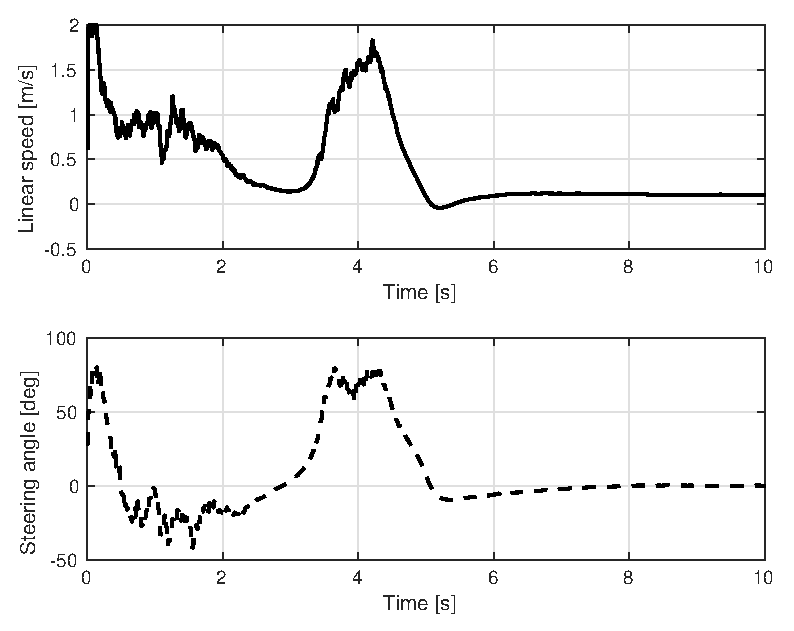
\includegraphics[width=0.48\textwidth,height=0.25\textheight]{figs/coppelia/firstScenario/controlInputRandomPathDistance.eps} }
 \subfigure[][]{%
    \label{fig:weightRandomDistance}%
    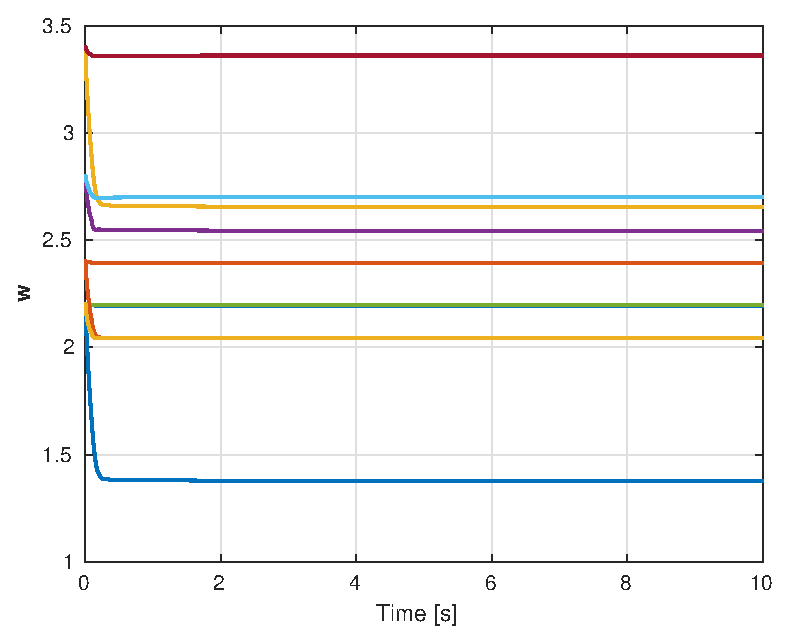
\includegraphics[width=0.48\textwidth,height=0.25\textheight]{figs/coppelia/firstScenario/weightRandomPathDistance.eps} }
\caption[Leader-follower performance for random trajectory.]{Performance in tracking random trajectory: 
  \subref{fig:trajectoryRandom} leader-follower trajectories,~\subref{fig:stateErrorRandom} state error,~\subref{fig:controlInputsRandom} linear speed and steering angle of the follower; and    \subref{fig:weightRandomDistance} learning weights.}%
  \label{fig:peformanceRandomTrajectory}%
\end{figure*}

% \textit{In the sequel, computer experiments  are conducted to validate the performance of the proposed model-free adaptive learning algorithm in real-time. The results of computer experiments highlight the dynamics of the tracking errors and the convergence characteristics of the proposed algorithm (i.e., updating the critic weights). This will judge the ability of the follower robot to track independent motion trajectory of the leader robot under two different independent leader-motion trajectories. The computer experiments are realized using MATLAB simulation environment. The weighting matrices are set to $\mathbf{Q} = \mathrm{diag}[0.01,0.01,0.005]$ and $\mathbf{R} = \mathrm{diag}[10^{-6}, 10^{-6}].$ % 
%  \[Q=0.001 
%  \begin{bmatrix}
%  10       & 0   & 0\\
%  0       & 10   & 0\\
%  0       & 0   &5 \\
%  \end{bmatrix},
%  R=0.000001
%  \begin{bmatrix}
%  1       & 0 \\
%  0       & 1 
%  \end{bmatrix}.\]
% The learning rate $\ell_c$ is set to  $0.0001$. The sampling time $T_s$ is set to $0.08 \sec.$ The desired distance offset between the leader and the follower is set to $ d = 0.5$ [m] for all scenarios.
%
%% In the first s\begin{figure*}[htbp]%
%\centering
%\parbox[c]{0.48\textwidth}{\centering Parallel parking}
%\parbox[c]{0.48\textwidth}{\centering Trajectory tracking}
%\\





% 
%%\begin{align*}
%% $\dot x^{[\ell]}(t) = \nu^{[\ell]}(t)\cos\theta^{[\ell]}(t),$ %
%% $\dot y^{[\ell]}(t) = \nu^{[\ell]}(t)\sin\theta^{[\ell]}(t).$
%% \dot\theta^\ell(t) &= \omega(t),
%%\end{align*}
% 
% Initially, the leader's position is set to be the same for a short period of time with $\nu^{\ell} = 0 , \gamma^{\ell} = 0$. Then it starts to move on a horizontal line with $\nu^{\ell} = 0.1 $ [m/s], eventually the leader starts to move on an inclined path with $\nu^{\ell} = 0.2$ [m/s], $\gamma^{\ell} = 45\degree$. The leader is initially placed at $(x,y) = (5, 2)~\si{[\meter]}$ with an orientation of $\theta = 0 \degree $, while the follower  is initially placed at $(x,y) = (0, 0)~\si{[\meter]}$ with an orientation of $\theta = 0\degree$. Note that during this scenario, the critic weights converge rapidly and the tracking errors decay till the follower tracks the leader. The trajectory phase plan plot, tracking error states, control signals, and tuning of critic weights are shown in Fig.~\ref{fig:performanceRectilinearTrajectory}. %
% 
%% \begin{figure*}[htbp]%
%%     \centering
%%     \parbox[c]{0.48\textwidth}{\centering Parallel parking}
%%     \parbox[c]{0.48\textwidth}{\centering Trajectory tracking}
%%     \\
%%     \subfigure[][]{%
%%         \label{fig:trajectoryRectilinearDistance}%
%%         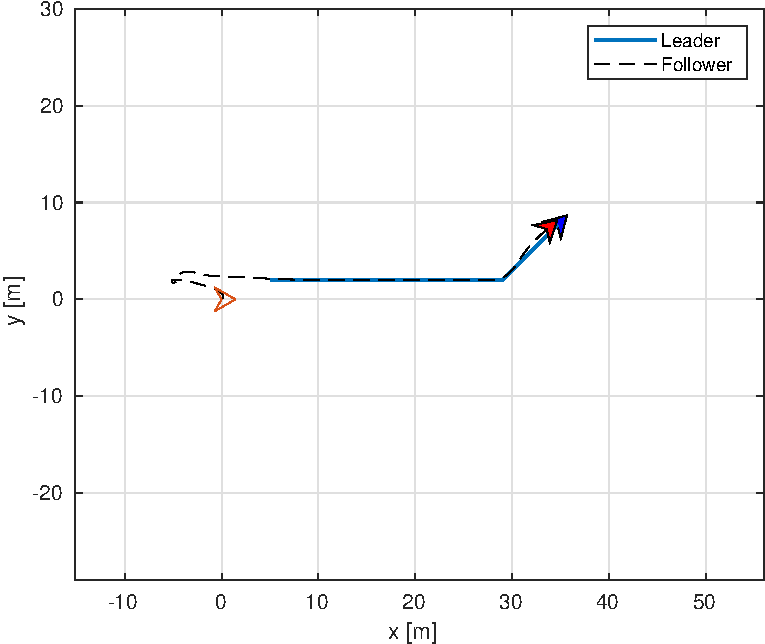
\includegraphics[width=0.48\textwidth,height=0.25\textheight]{figs/matlab/rectilinear/trajectoryRectlinearDistance} }
%%     \subfigure[][]{%
%%         \label{fig:stateErrorRectilinearDistance}%
%%         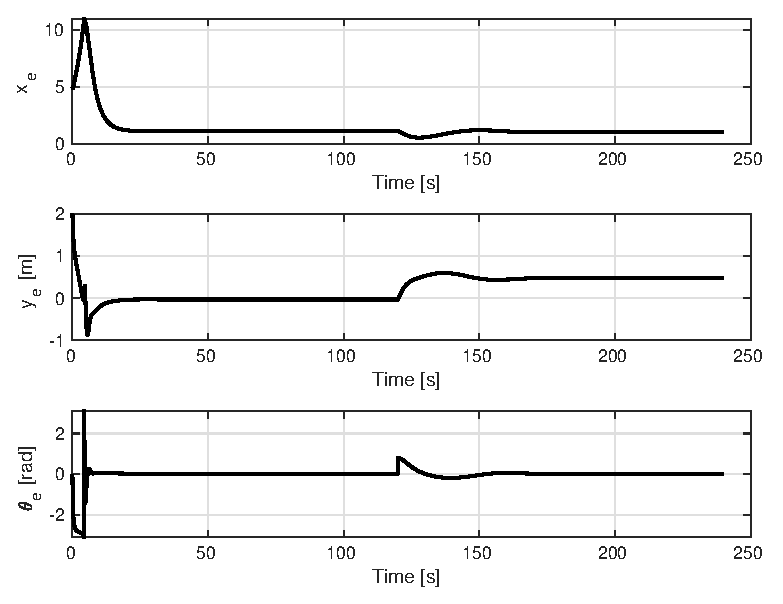
\includegraphics[width=0.48\textwidth,height=0.25\textheight]{figs/matlab/rectilinear/stateErrorRectlinearDistance} }
%%     \\
%%     \subfigure[][]{%
%%         \label{fig:controlInputsRectilinearDistance}%
%%         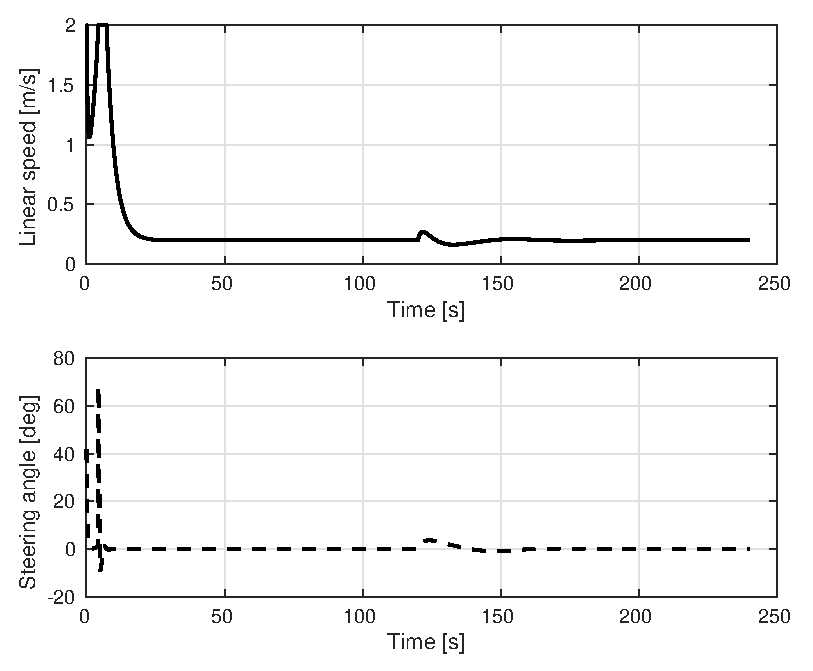
\includegraphics[width=0.48\textwidth,height=0.25\textheight]{figs/matlab/rectilinear/controlInputRectlinearDistance} }
%%     \subfigure[][]{%
%%         \label{fig:weightRectilinearDistance}%
%%         \includegraphics[width=0.48\textwidth,height=0.25\textheight]{figs/matlab/rectilinear/weightRectilinearDistance} }
%%     \caption[Leader-follower performance for rectilinear trajectory.]{First scenario (rectilinear trajectory): 
%%         \subref{fig:trajectoryRectilinearDistance} leader-follower trajectories,~\subref{fig:stateErrorRectilinearDistance} state tracking errors,~\subref{fig:controlInputsRectilinearDistance} linear speed and steering angle of the follower, and    \subref{fig:weightRectilinearDistance} critic weights.}%
%%     \label{fig:performanceRectilinearTrajectory}%
%% \end{figure*}
% 
%
%
% A relatively unplanned complex trajectory-tracking scenario is considered. The leader moves according to a sinusoidal trajectory so that %
% 
%%  \begin{align*}
%% $x^{[\ell]}(t) = \alpha (t) \in [0,10\pi],$ %
%% $y^{[\ell]}(t) = 5 \,\sin(\alpha t),$ and %
%% $\theta^{[\ell]}(t) = cos(\alpha t).$  %
%%        \end{align*}
%% 
% The leader robot  was initially placed at $(x,y) = (0, 0)~\si{[\meter]}$ with an orientation of $\theta = 0 \degree$ while the follower robot was initially placed at a random position around $(x,y) = (0, 0)~\si{[\meter]}$ with a random orientation. The simulation results are summarized in Figure~\ref{fig:performanceSinewaveTrajectory}. It is observed that the critic weights take more time to converge compared to the earlier scenario,  which is reluctant to the complexity of the independent trajectory of the leader. This result emphasizes the adaptability of the proposed adaptive learning mechanism to different scenarios. Further, the follower starts to move away from the leader at the beginning of the simulation before it finally converges to the leader where the tracking errors are bounded by a safe distance $d.$ % 
% 
%% \begin{figure*}[htbp]%
%%     \centering
%%     \parbox[c]{0.48\textwidth}{\centering Parallel parking}
%%     \parbox[c]{0.48\textwidth}{\centering Trajectory tracking}
%%     \\
%%     \subfigure[][]{%
%%         \label{fig:trajectorySinewave}%
%%         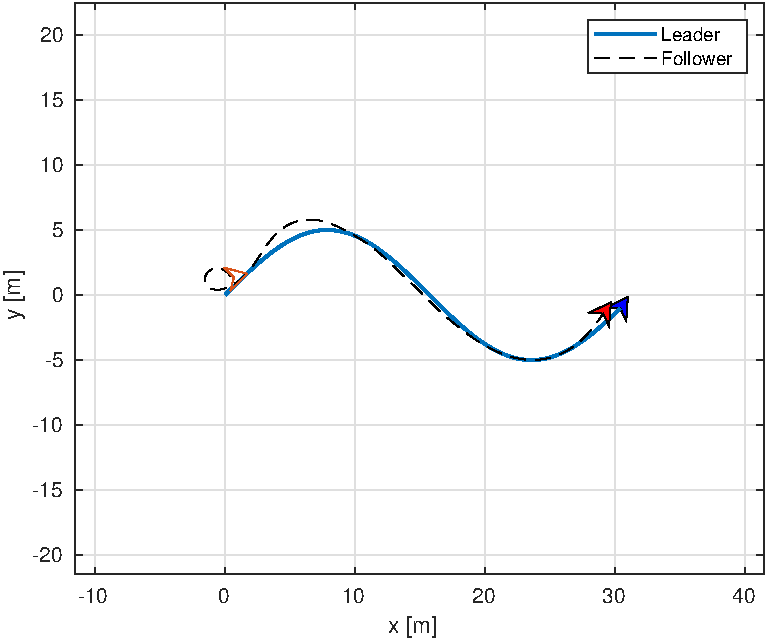
\includegraphics[width=0.48\textwidth,height=0.25\textheight]{figs/matlab/sinewave/trajectorySinewaveDistance} }
%%     \subfigure[][]{%
%%         \label{fig:stateErrorSinewave}%
%%         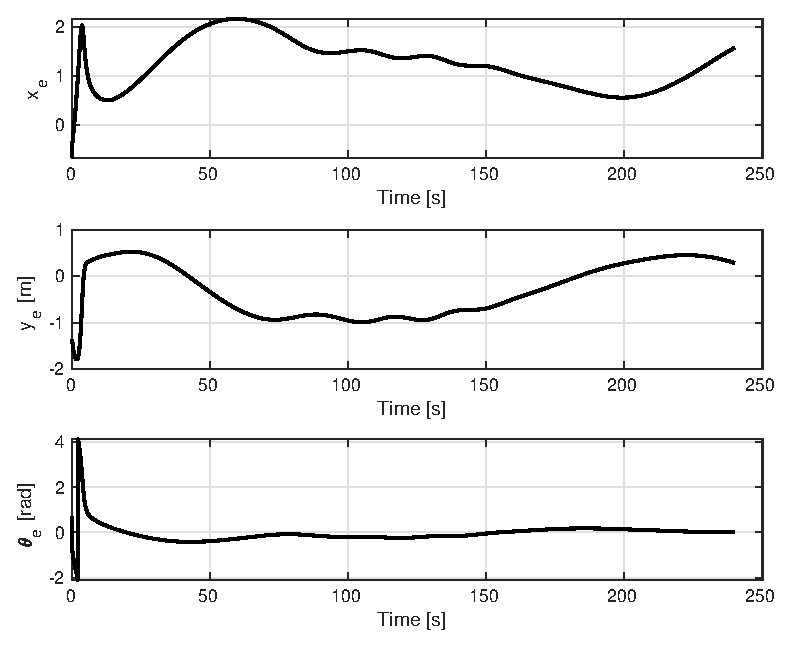
\includegraphics[width=0.48\textwidth,height=0.25\textheight]{figs/matlab/sinewave/stateErrorSinewaveDistance} }
%%     \\
%%     \subfigure[][]{%
%%         \label{fig:controlInputSinewave}%
%%         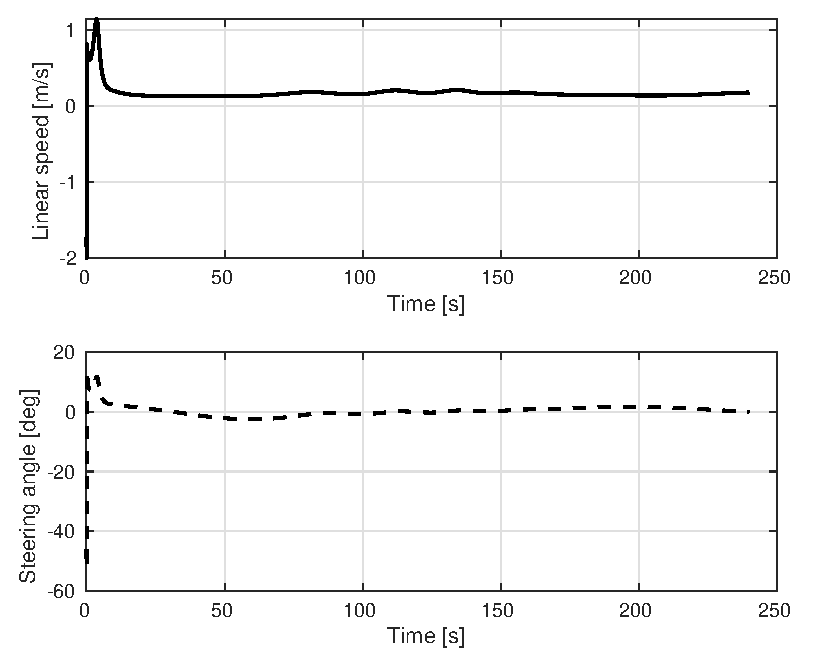
\includegraphics[width=0.48\textwidth,height=0.25\textheight]{figs/matlab/sinewave/controlInputSinewaveDistance} }
%%     \subfigure[][]{%
%%         \label{fig:weightSinewaveDistance}%
%%         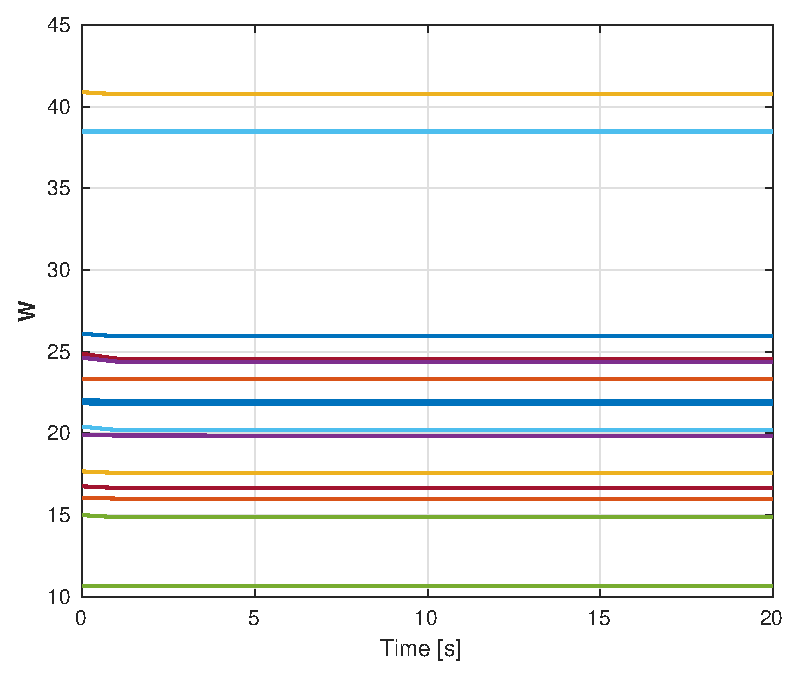
\includegraphics[width=0.48\textwidth,height=0.25\textheight]{figs/matlab/sinewave/weightSinewaveDistance} }
%%     \caption[Leader-follower performance for nonlinear trajectory.]{Second scenario (sinusoidal trajectory): 
%%         \subref{fig:trajectorySinewave} leader-follower trajectories,~\subref{fig:stateErrorSinewave} state tracking errors,~\subref{fig:controlInputSinewave} linear speed and steering angle of the follower, and    \subref{fig:weightSinewaveDistance} critic weights.}%
%%     \label{fig:performanceSinewaveTrajectory}%
%% \end{figure*}
% 
%
%
%\textit{In the third case study we rely on completley random path for the leader robot to evaluate the effectivenss of the proposed algorithm as a solution for the leader follower tracking problem. The leader is to follow a random path defined by the model described in (2), with $\gamma$ being a random value, The follwer is to maitain an offset distance of $d = 0.5 $ [m]. Note that the path of the leader is not pre defined and the algorithm being completlety model free. The results are summerized in Fig. \ref{fig:peformanceRandomTrajectory}. }


%The results are summarized in Fig.~\ref{fig:peformanceRandomTrajectory}. %
%
%\begin{figure*}[htbp]%
%\centering
%\parbox[c]{0.48\textwidth}{\centering Parallel parking}
%\parbox[c]{0.48\textwidth}{\centering Trajectory tracking}
%\\
%\subfigure[][]{%
%    \label{fig:trajectoryRandom}%
%    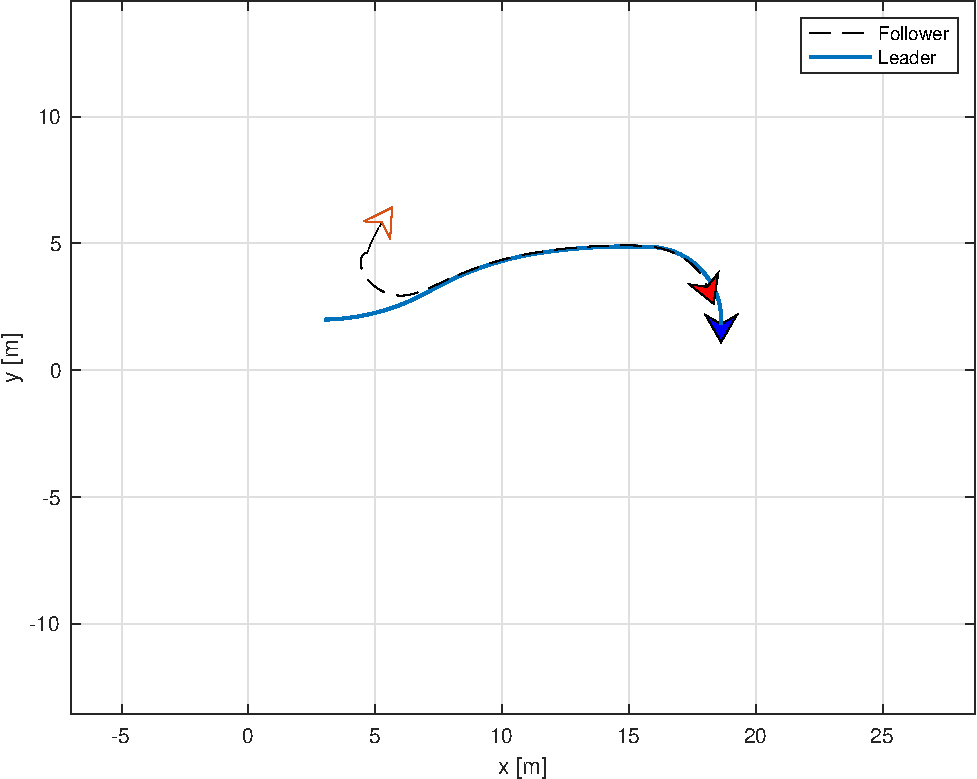
\includegraphics[width=0.48\textwidth,height=0.25\textheight]{figs/matlab/randomPath/trajectorySinewave} }
%\subfigure[][]{%
%    \label{fig:stateErrorRandom}%
%    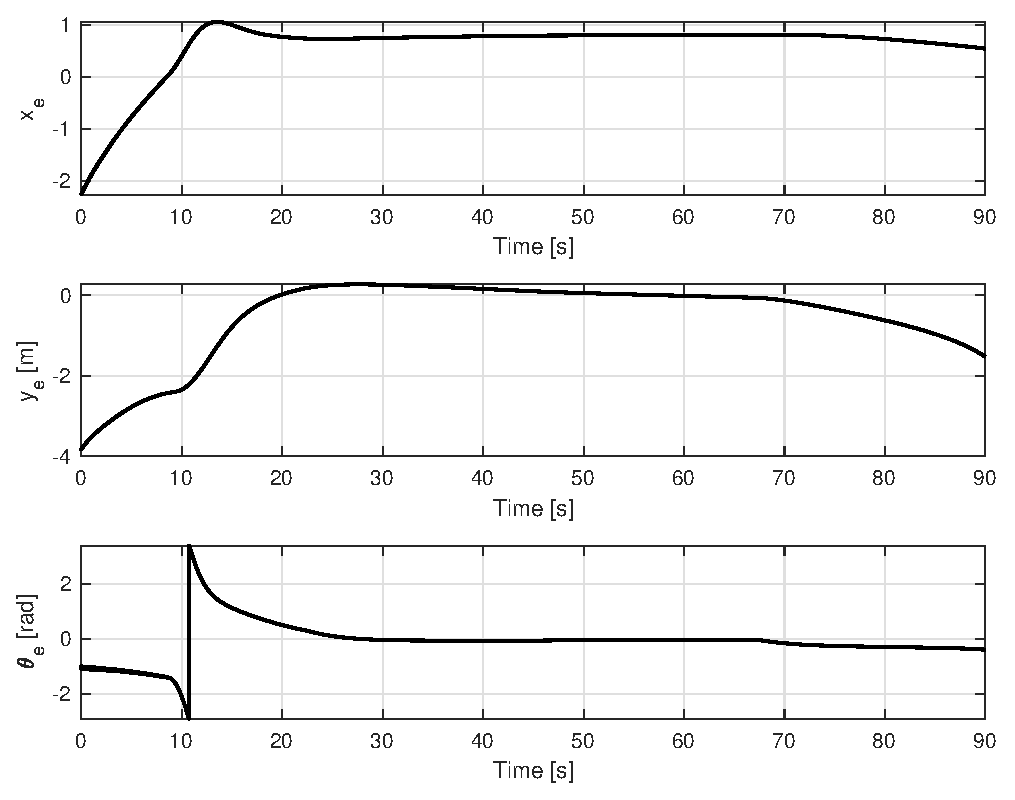
\includegraphics[width=0.48\textwidth,height=0.25\textheight]{figs/matlab/randomPath/stateErrorSinewave} }
%\\
% \subfigure[][]{%
%    \label{fig:controlInputsRandom}%
%    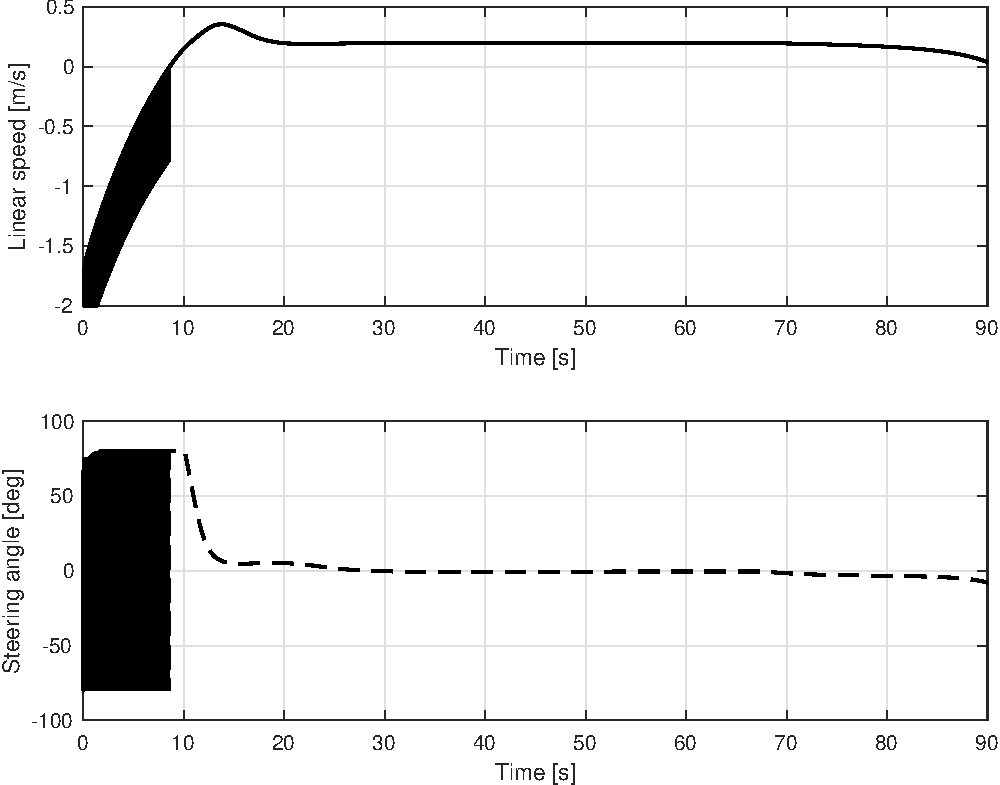
\includegraphics[width=0.48\textwidth,height=0.25\textheight]{figs/matlab/randomPath/controlInputSinewave} }
% \subfigure[][]{%
%    \label{fig:weightRandomDistance}%
%    \includegraphics[width=0.48\textwidth,height=0.25\textheight]{figs/matlab/randomPath/weightRectilinearDistance} }
%\caption[Leader-follower performance for random trajectory.]{Performance in tracking random trajectory: 
%  \subref{fig:trajectoryRandom} leader-follower trajectories,~\subref{fig:stateErrorRandom} state error,~\subref{fig:controlInputsRandom} linear speed and steering angle of the follower; and    \subref{fig:weightRandomDistance} learning weights.}%
%  \label{fig:peformanceRandomTrajectory}%
%\end{figure*}



 \section{Conclusion} \label{sec:conclusion}

% A novel policy iteration mechanism based on a model-free reinforcement learning approach is presented for solving a conventional leader-follower formation problem using car-like mobile robots. The proposed approach does not rely on model parameters inherent in the mobile robots employed in this work. The follower robot is able to follow the leader robot that navigates along unplanned trajectories of various complexities while maintaining a nonzero safe distance between them. To the best of authors' knowledge, this is the first milestone of its kind where a model-free policy iteration based reinforcement learning approach is employed in a multi-robot formation control problem. The future work is going  to extend the learning algorithm for solving a time-varying formation control problem using networked robots.

% \section*{Acknowledgment}

% The preferred spelling of the word ``acknowledgment'' in America is without 
 an ``e'' after the ``g''. Avoid the stilted expression ``one of us (R. B. 
 G.) thanks $\ldots$''. Instead, try ``R. B. G. thanks$\ldots$''. Put sponsor 
 acknowledgments in the unnumbered footnote on the first page.



 \bibliographystyle{IEEEtran}
\bibliography{bib/refsSuruzWeb,bib/refsMultiAgent,bib/refsRoboticsJournals,bib/refsRoboticsConferences,bib/refsGenericControl,bib/refsBooksTRTheses,bib/refsReinforcementLearningADP,bib/refsRL-Keshtkar}
\end{document}

%%% Local Variables:
%%% mode: latex
%%% TeX-master: t
%%% End:
